\documentclass[11pt,a4paper]{article}
\usepackage[T1]{fontenc}
\usepackage{lmodern}
\usepackage{xcolor}
\usepackage{titlesec}
\usepackage{geometry}
\usepackage{natbib}
\usepackage{enumitem}
\usepackage{hyperref}
\usepackage{graphicx}
\usepackage{caption}
\usepackage{booktabs}
\usepackage{amsmath}
\usepackage{subcaption}

\definecolor{primary}{RGB}{0,103,149}
\definecolor{secondary}{RGB}{128,179,211}

\geometry{margin=2.5cm}

\titleformat{\section}
  {\color{primary}\Large\bfseries}
  {\thesection}{1em}{}[\titlerule]
\titleformat{\subsection}
  {\color{primary}\large\bfseries}
  {\thesubsection}{1em}{}

\hypersetup{
    colorlinks=true,
    linkcolor=primary,
    urlcolor=primary,
    citecolor=primary
}

\linespread{1.15}

\begin{document}

\title{\textcolor{primary}{\textbf{“Beyond the Price Tag: Examining User Behavior and Trust in Free VPN Services”}}}
\author{Kurudunje Deekshith Shetty | Shitil Shetty}
\date{9th May, 2025}
\maketitle

\begin{abstract}
This study investigates user trust in free Virtual Private Network (VPN) services through a primary survey of 94 general users, complemented by a secondary survey of 16 security-aware users with cybersecurity expertise. Results reveal a pronounced privacy paradox: general users, driven by cost, adopt free VPNs despite low trust and limited understanding of data practices, while security-aware users, critical of technical vulnerabilities, prefer paid alternatives. Detailed analysis of usage patterns, trust levels, motivations, issues, and perceived risks underscores the need for enhanced transparency and user education to align VPN usage with privacy goals.
\end{abstract}

\section{Introduction}
Virtual Private Networks (VPNs) are critical for enhancing online privacy and security by encrypting traffic and masking IP addresses to mitigate surveillance and data breaches \citep{Mehrnezhad2022, Alshalan2016}. Free VPN services, while popular, raise concerns due to their reliance on data monetization or compromised security \citep{Ikram2016, Khan2018}. This research examines user trust in free VPNs through a primary survey of 94 general users conducted in April 2025, supplemented by a secondary survey of 16 security-aware users (April 11--19, 2025) offering technical insights \citep{Shetty2025}. The study addresses four key research questions:

\begin{itemize}
   
    \item To what extent do users understand and trust free VPN providers' data handling practices?
    \item What motivates users to choose free VPNs over paid alternatives?
    \item What issues do users commonly experience with free VPN services?
    \item What are users' perceptions of risks associated with free VPNs and how import is data privacy to them?
\end{itemize}

By contrasting general and security-aware user perspectives, this study provides a nuanced understanding of trust dynamics, informing strategies to improve the VPN ecosystem.

\section{Background and Related Work}
Global VPN adoption has surged amid growing privacy concerns \citep{Dutkowska2022, Moore2024}. Research identifies a ``privacy paradox,'' where users prioritize convenience over security, often choosing free VPNs despite risks \citep{Story2021, Namara2020}. Free VPNs frequently monetize user data or exhibit vulnerabilities like weak encryption \citep{Khan2018, Wilson2020}.

Technical analyses highlight implementation flaws, such as inadequate encryption or data logging \citep{Abbas2023, Ramesh2022}, while user studies explore adoption factors like cost and ease of use \citep{Sombatruang2020, Blancaflor2024}. Foundational surveys provide insights into VPN technologies \citep{Erdogan2008, Khanvilkar2004}, and recent work examines specific use cases, such as secure communications \citep{Fassl2023, Singh2016}. 

This study builds on these efforts by integrating general user data with security-aware perspectives from a complementary survey \citep{Shetty2025}, offering a comprehensive view of trust and behavior in free VPN usage.

\section{Methods}
The study utilized a dual-survey methodology:

\begin{enumerate}
    \item \textbf{General User Survey}: Conducted in April 2025 with 94 participants , this survey included 22 questions on demographics, VPN usage, trust, motivations, issues, and risks. It featured multiple-choice, Likert-scale, and open-ended questions, capturing diverse user experiences which was shared through social media platforms like reddit and LinkedIn.
    \item \textbf{Security-Aware User Survey}: Conducted April 11--19, 2025, with 16 participants/students undertaking Human Factors in Security course, this survey focused on technical evaluations, trust factors, and security concerns\citep{Shetty2025}.
\end{enumerate}

Quantitative data were analyzed using descriptive statistics, while qualitative responses were thematically coded to identify recurring patterns. Participants were anonymized (P1--P94 for general users, aliases like ``cranky-wilbur'' for security-aware users).

\section{Results and Analysis}
The following subsections address the research questions, integrating insights from both surveys and highlighting key trends from the general user data.

\subsection{Demographic Characteristics}
The general user sample was predominantly young (61.7\% aged 18--24, 24.5\% 25--34, 13.9\% other), gender-balanced (46.8\% male, 51\% female, 2.2\% non-binary), and moderately educated (43.6\% bachelor’s, 26.6\% master’s or higher). Technical proficiency was mostly intermediate (67\%), with 18.1\% beginners and 14.9\% advanced.

Security-aware users were with higher proficiency (25\% advanced, 12.5\% expert) and roles such as cybersecurity analysts, software developers, and students \citep{Shetty2025}. Their technical expertise shaped their critical stance on free VPNs.

\subsection{VPN Usage Patterns}
Among general users, 41.5\% (39) used free VPNs, 17\% (16) used paid VPNs, and 41.5\% (39) used none. Usage frequency varied: 40\% of free VPN users were daily users, 35\% weekly, and 25\% monthly or less. Common activities included anonymous browsing (52.6\%, 41 responses), streaming geo-restricted content (34.6\%, 27), remote work (17.9\%, 14), gaming (17.9\%, 14), and accessing restricted websites (19.2\%, 15). Notably, 63.8\% (60) never used VPNs for sensitive tasks (e.g., online banking), with only 3.2\% (3) reporting frequent use, indicating limited trust in free VPNs for critical tasks.

Survey responses revealed specific use cases, such as P8 using free VPNs for ``international shows'' and P6 for ``remote work,'' reflecting entertainment and professional needs. Non-users cited reasons like perceived illegality (P7: ``It’s illegal'') or lack of need (P18: ``Not really sure what it is'').

Security-aware users showed a distinct pattern: 43.8\% (7) used paid VPNs, 18.8\% (3) used free VPNs, and 37.5\% (6) used none \citep{Shetty2025}. They prioritized secure communications and restricted network access, using free VPNs only for low-risk tasks, as noted by ``goofy-liskov'': ``a quick and easy solution'' for non-critical scenarios.

\begin{figure}[ht]
    \centering
    \begin{subfigure}[b]{1.0\columnwidth}
        \centering
        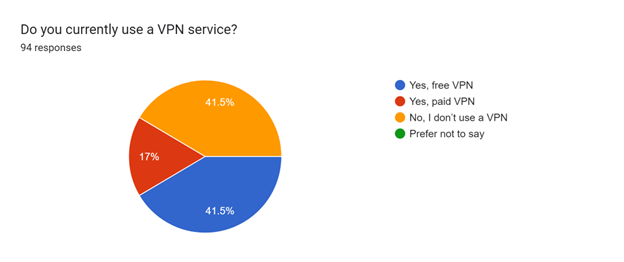
\includegraphics[width=\textwidth]{general user vpn usage.png}
        \caption{General Users}
        \label{fig:general_users_usage}
    \end{subfigure}
    \hfill
    \begin{subfigure}[b]{1.0\columnwidth}
        \centering
        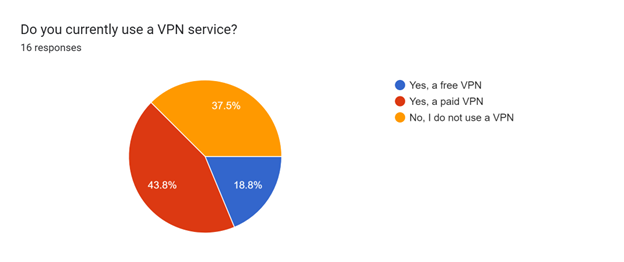
\includegraphics[width=\textwidth]{security aware usage.png}
        \caption{Security-Aware Users}
        \label{fig:security_aware_usage}
    \end{subfigure}
    \caption{VPN usage distribution: general users (41.5\% free, 17\% paid, 41.5\% none) versus security-aware users (18.8\% free, 43.8\% paid, 37.5\% none), highlighting technical users' preference for paid services.}
    \label{fig:vpn_usage}
\end{figure}

Figure~\ref{fig:vpn_usage} underscores security-aware users’ preference for paid VPNs, driven by reliability concerns \citep{Ramesh2023}.

\subsection{Trust and Understanding of Data Practices}
Trust in free VPN providers was low among general users: 30.9\% (29) reported minimal trust, 37.2\% (35) were neutral, 16\% (15) had moderate trust, and 1.1\% (1) expressed complete trust on a 5-point scale. Understanding of data practices was limited, with 48.9\% (46) unsure of providers’ handling, 19.1\% (18) believing data is collected and shared with third parties, 19.1\% (18) assuming collection without selling, and 9.6\% (9) believing no data is collected.

Engagement with terms and conditions was minimal, with 46.5\% (40) never reviewing them. Among the 34.9\% (30) who did, comprehension varied: 24\% (22) reported partial understanding (2--3/5), and 8.8\% (5) reported full understanding (4--5/5). For example, P17, who reviewed terms thoroughly, noted a clear need for ``A transparent privacy policy that states they don't log, track, or sell user data, a reputation and track record for privacy above all else, and a clear idea of how the provider makes their money without selling user data.'' to build trust. 

Security-aware users exhibited lower trust, with 37.5\% (6) rating trust at 1/5, 37.5\% (6) at 2/5, and 25\% (4) at 3/5, none exceeding neutral \citep{Shetty2025}. They assumed data collection, citing specific data types like ``browsing history, connection logs'' (``ecstatic-cori'') and ``traffic, fingerprints'' (``infallible-lalande''). Their scrutiny of terms revealed dissatisfaction with vague policies, with ``trusting-mahavira'' questioning whether VPNs ''truly keep no logs.''

\begin{figure}[ht]
    \centering
    \begin{subfigure}[t]{1.0\columnwidth}
        \centering
        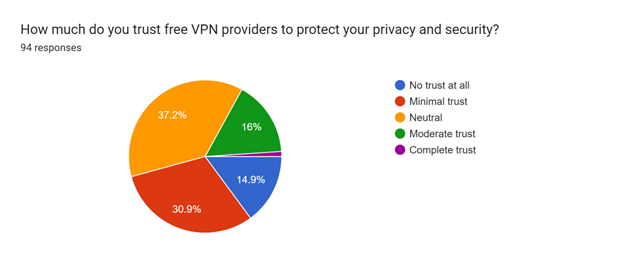
\includegraphics[width=\linewidth]{generalusertrust.png}
        \caption{General Users}
        \label{fig:general_trust}
    \end{subfigure}
    \hfill
    \begin{subfigure}[t]{1.0\columnwidth}
        \centering
        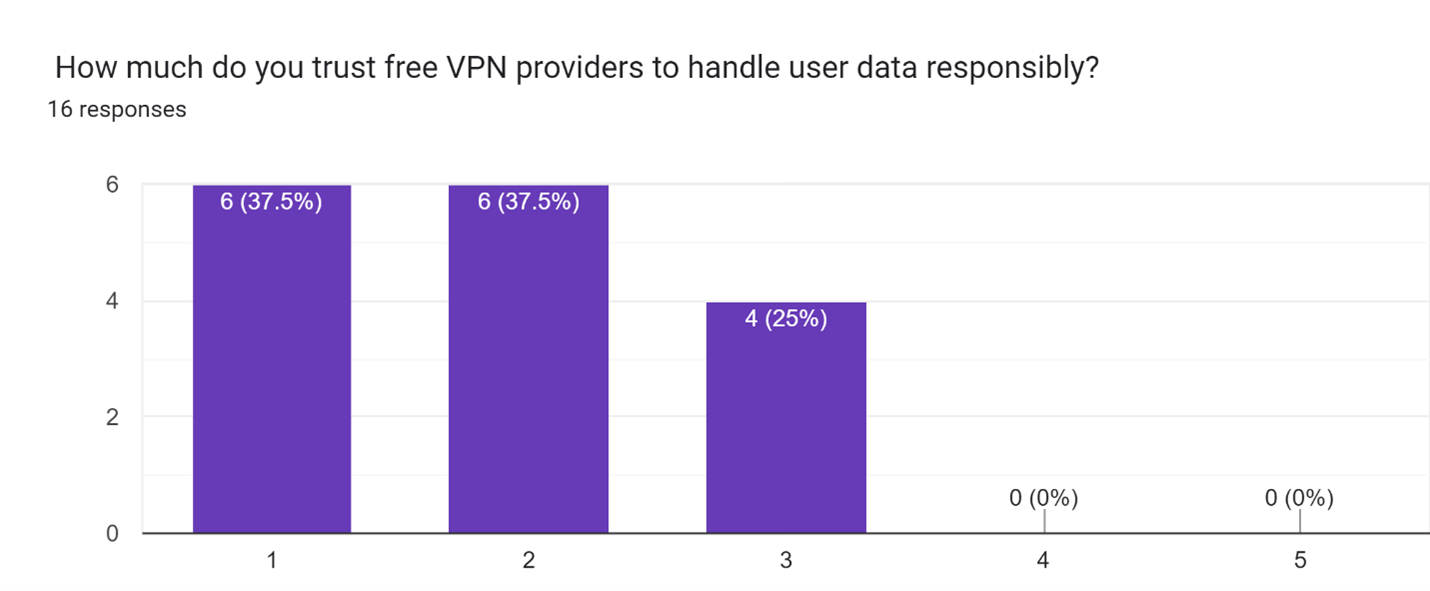
\includegraphics[width=\linewidth]{securityusertrust.png}
        \caption{Security-Aware Users}
        \label{fig:security_trust}
    \end{subfigure}
    \caption{Trust levels in free VPN providers: general users (30.9\% minimal trust) versus security-aware users (37.5\% at 1/5, none above 3/5), highlighting greater skepticism among technical users.}
    \label{fig:trust_levels_comparison}
\end{figure}

Figure~\ref{fig:trust_levels_comparison} illustrates the trust gap, amplified by security-aware users’ awareness of data risks \citep{Ikram2016, Khan2018}.
\subsection{Motivations for Choosing Free VPNs}
Cost was the primary motivator for general users (73.5\%, 61 responses), followed by ease of access (33.7\%, 28), lack of awareness of paid options (14.5\%, 12), trialing before purchase (14.5\%, 12), and trust in providers (6\%, 5). Among free VPN users, 87.2\% (34 of 39) cited cost, reflecting economic constraints, particularly among younger users (e.g., P15: ``Cost (free service)'').

Survey responses highlighted economic drivers, with P13 noting free VPNs as a way to avoid ``spending a lot of money on subscriptions.'' Lack of awareness was evident in P11’s choice through their statement ``lack of awareness about paid options.''

Security-aware users using free VPNs (3 respondents) cited convenience for non-critical tasks, with ``goofy-liskov'' emphasizing their use as a ``quick solution'' despite risks \citep{Shetty2025}.

\begin{table}[ht]
    \centering
    \caption{Motivations for Choosing Free VPNs Among General Users}
    \begin{tabular}{lc}
        \toprule
        \textbf{Motivation} & \textbf{Frequency (\%)} \\
        \midrule
        Cost & 61 (73.5\%) \\
        Ease of Access & 28 (33.7\%) \\
        Lack of Awareness & 12 (14.5\%) \\
        Trialing & 12 (14.5\%) \\
        Trust in Provider & 5 (6\%) \\
        \bottomrule
    \end{tabular}
    \caption*{Frequency of motivations for selecting free VPNs among general users, with cost dominating at 73.5\%.}
    \label{tab:motivations}
\end{table}

Table~\ref{tab:motivations} underscores economic incentives, consistent with prior findings \citep{Namara2020, Sombatruang2020}.

\subsection{Common Issues}
General users reported frequent issues with free VPNs: slow speeds (51.2\%, 44 responses), disconnections (40.7\%, 35), invasive advertisements (23.3\%, 20), privacy concerns (9.3\%, 8), and malware or viruses (7\%, 6). Among free VPN users, 58.9\% (23 of 39) experienced slow speeds, and 46.2\% (18) reported disconnections, impacting usability (e.g., P5: ``Data speed gets reduced'').

Survey responses emphasized performance issues, with P3 noting ``frequent disconnections'' and P9 citing ``invasive advertisements'' as deterrents.

Security-aware users echoed performance concerns but emphasized technical vulnerabilities: weak encryption (68.8\%, 11 responses), malware risks (62.5\%, 10), and data logging (93.8\%, 15) and surprisingly all the participants were concerned with VPNs selling user data to third parties (100 \%, 16)\citep{Shetty2025}. Table~\ref{tab:issues} summarizes general users issues.

\begin{table}[ht]
    \centering
    \caption{Common Issues with Free VPNs}
    \begin{tabular}{lcc}
        \toprule
        \textbf{Issue} & \textbf{General Users (\%)}\\
        \midrule
        Slow Speeds & 44 (51.2\%) \\
        Disconnections & 35 (40.7\%) \\
        Advertisements & 20 (23.3\%) \\
        Weak Encryption & 3 (3.2\%)\\
        Malware Risks & 6 (7\%) \\
        Privacy Concerns & 8 (9.3\%) \\
        \bottomrule
    \end{tabular}
    \label{tab:issues}
\end{table}

The overlap in performance complaints suggests universal usability challenges, while security-aware users’ focus on encryption and malware reflects deeper risk awareness \citep{Wilson2020, Ramesh2022}.

\subsection{Perceived Risks and Trust Factors}
Data privacy was the primary concern for general users (35.9\%, 33 responses), with P17 stating: ''Everything you do through an untrustworthy free VPN… should be expected to be monitored, tracked, and sold.'' Other risks included security vulnerabilities (15.2\%, 14; P13: ``Lack of security''), performance issues (10.9\%, 10; P15: ``Slow data''), scams (8.7\%, 8; P11: ``Scam''), and data breaches (6.5\%, 6; P12: ``Data hack'').

Transparency was critical, with 37.2\% (35) rating it ''absolutely essential'' and 30.9\% (29) ''very important.'' Open-ended responses emphasized clear policies (P17: ''A transparent privacy policy''), better security (13\%, 12; P11: ''Better security''), and user-accessible data logs (8.7\%, 8; P19: 'Making the data available to the user'').

Security-aware users focused on data logging (93.8\%, 15; ''cranky-wilbur'': ''data collection, hidden tracking, selling user data''), weak encryption (68.8\%, 11; ''trusting-mahavira'': ''how strong and up-to-date the VPN encryption is''), and malware (62.5\%, 10; ''ecstatic-cori'': ''VPNs don’t protect against malware'') \citep{Shetty2025}. They demanded technical assurances: public audits (75\%, 12), open-source code (68.8\%, 11), and no-ads policies (50\%, 8).

\begin{figure}[ht]
    \centering
    \begin{subfigure}[t]{1.0\columnwidth}
        \centering
        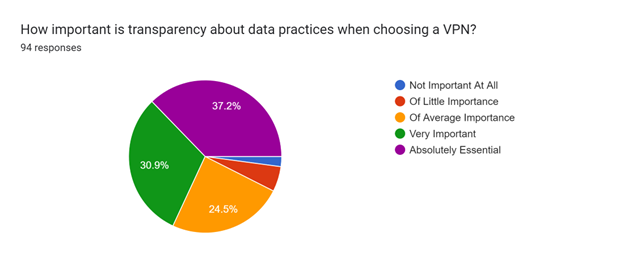
\includegraphics[width=\linewidth]{generaluserimportance.png}
        \caption{General Users}
        \label{fig:general_risks}
    \end{subfigure}
    \hfill
    \begin{subfigure}[t]{1.0\columnwidth}
        \centering
        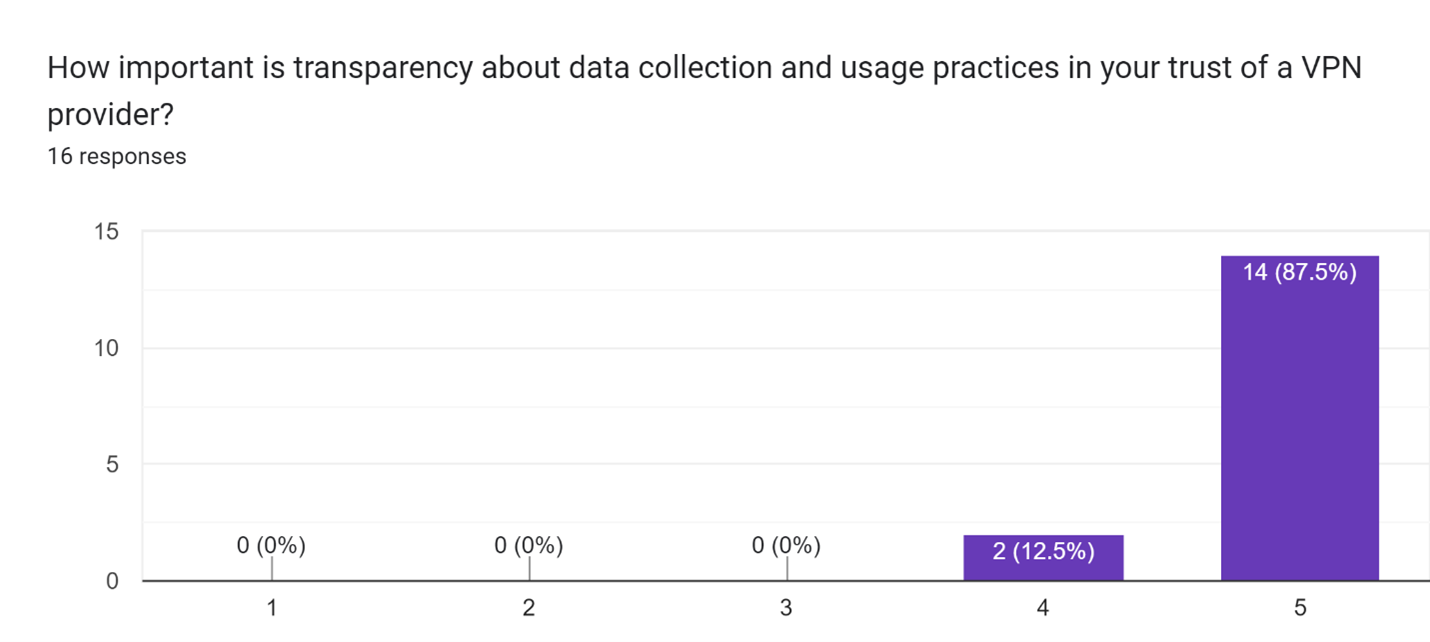
\includegraphics[width=\linewidth]{importancesecurityaware.png}
        \caption{Security-Aware Users}
        \label{fig:security_risks}
    \end{subfigure}
    \caption{Transparency in free VPNs (Rated "Absolutely Essential"): general users (37.2\%) versus security-aware users (87.5\%).}
    \label{fig:risks_comparison}
\end{figure}

Figure~\ref{fig:risks_comparison} highlights the importance of transparency and privacy.

\subsection{Additional Insights: Recommendations and Knowledge Gaps}
Security-aware users were reluctant to recommend free VPNs to non-technical peers, with 43.8\% (7) rating it ''very unlikely'' and 25\% (4) ''unlikely,'' citing risks like ``a false sense of security'' (``interesting-buck'') \citep{Shetty2025}. They emphasized security protocols and logging policies over ease of use (''cranky-wilbur'').

General users showed limited awareness, with 13\% (12) citing unfamiliarity with paid options and 48.9\% (46) unsure of data practices. Responses like P18’s (''not really sure what it is'') and P23’s (``no idea what a VPN is'') highlight an education gap.

Security-aware users’ high VPN knowledge (75\% at 4/5 or higher) shaped their concerns about data monetization (``funny-golick'': ``Free VPNs likely use your traffic and device information to sell to others'') \citep{Shetty2025}.

\section{Discussion}
The findings confirm a privacy paradox among general users: cost (73.5\%) drives free VPN adoption despite low trust (45.8\% "No tust and minimal trust") and poor understanding (35\%, 1--2/5) \citep{Story2021, Namara2020}. Security-aware users, aware of technical flaws like data logging (93.8\%) and weak encryption (68.8\%) \citep{Khan2018, Ramesh2022, Shetty2025}, prefer paid VPNs (43.8\%), illustrating knowledge-driven behavior.

The universal demand for transparency (37.2\% general users, 100\% security-aware users rating it 4/5 or higher) suggests providers could build trust through clear policies, audits, and open-source code \citep{Blancaflor2024, Abbas2023}. Limited engagement with terms (71\%) and widespread uncertainty underscore an education gap \citep{PriyankaP15, Story2021}.

General users’ reliance on free VPNs for entertainment (52.6\% browsing, 34.6\% streaming) and avoidance of sensitive tasks (63.8\%) reflect pragmatic but risky choices. Security-aware users’ technical critiques and preference for paid VPNs suggest education could shift general users toward safer options \citep{Sombatruang2020, Singh2016}.

\subsection{Limitations}

The general user survey’s skew toward younger participants (61.7\% aged 18--24) may underrepresent older demographics’ VPN trust and usage patterns, limiting applicability to broader populations. The security-aware survey’s small sample (16 participants) restricts statistical robustness, potentially missing nuanced technical perspectives. Self-reported data, particularly from general users, may reflect recall inaccuracies or social desirability bias, especially on sensitive topics like privacy concerns. Future studies should target balanced age distributions, expand the security-aware cohort, and incorporate objective measures, such as VPN log analyses or penetration testing, to validate user-reported issues \citep{Ramesh2022, Wilson2020}.

\section{Conclusion}
This study rigorously examines trust in free VPN services by comparing 94 general users and 16 security-aware users. General users, predominantly aged 18--24 (61.7\%) and motivated by cost (73.8\%), use free VPNs primarily for anonymous browsing (52.6\%) and streaming geo-restricted content (34.6\%), yet exhibit low trust (45.8\% minimal) and limited understanding of data practices (47.8\% unsure). Security-aware users, with advanced (50\%) or expert (25\%) cybersecurity skills, favor paid VPNs (43.8\%) and critique free VPNs for specific vulnerabilities, including data logging and outdated encryption protocols \citep{Shetty2025}. The findings directly address the research questions:

\begin{itemize}
    \item \textbf{Demographics and Usage}: Free VPN users are young and entertainment-driven, while security-aware users focus on secure communications for professional tasks.
    \item \textbf{Trust}: General users’ uncertainty contrasts with security-aware users’ informed skepticism about data handling and encryption weaknesses.
    \item \textbf{Motivations}: Cost drives general users, whereas security-aware users restrict free VPN use to low-stakes activities like casual browsing.
    \item \textbf{Issues}: Slow speeds (51.2\%) and disconnections plague general users, while security-aware users highlight risks like unencrypted traffic.
    \item \textbf{Risks}: Both groups prioritize data privacy, with security-aware users pinpointing threats like third-party data sharing.
    \item \textbf{Recommendations}: Both groups steadily support transparency about the data practices. 
\end{itemize}

Future research should develop targeted educational campaigns to improve general users’ understanding of VPN data practices, assess the viability of ad-supported VPN models that prioritize privacy, and evaluate the impact of mandatory third-party security audits on user trust \citep{Namara2020, Xu2020, Dutkowska2022}.

\bibliographystyle{plain}
\bibliography{references}

\end{document}